\section*{Теория}

\textit{Скин-эффектом} называется явление протекания токов высокой частоты в тонком поверхностном слое проводника. Скин-эффект проявляется в виде уменьшения амплитуды колебаний внутри проводника и увеличении в поверхностном слое.

Качественно скин-эффект объясняется явлением электромагнитной индукции. Рассмотрим длинный цилиндрический проводник (рис. \ref{fig:emi}), по которому течет ток $J$. Согласно закону Био-Савара-Лапласа, электрический ток создает магнитное поле $B$, силовые линии которого представляют собой окружности с центром на оси проводника.

\begin{figure}[H]
	\centering
	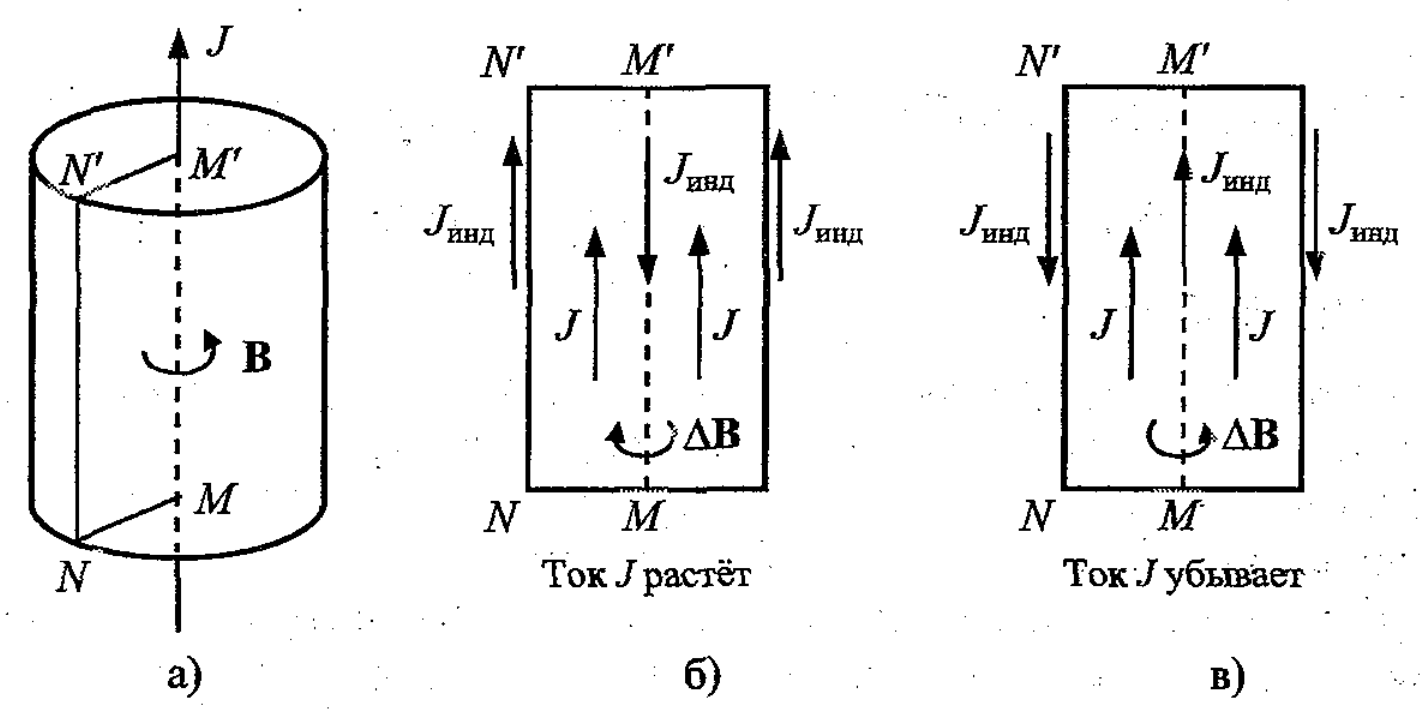
\includegraphics[width=0.7\textwidth]{../res/emi.png}
	\caption{а) -- переменный ток внутри проводника. б) и в) -- случаи увеличения и уменьшения тока.}
	\label{fig:emi}
\end{figure}

Рассмотрим контур $NMM'N'$ внутри проводника. По закону электромагнитной индукции при изменении магнитного потока сквозь этот контур, создаётся индукционное электрическое поле:
$$
	\oint\limits_\Gamma \pmb{E}_{инд} \,d\pmb{l} = - \int\limits_S \frac{\partial \pmb{B}}{\partial t} d\pmb{S}
$$
При возрастании тока через проводник $\frac{d J}{dt} > 0$, индукционный ток сонаправлен с внешним током на отрезке $NN'$ и противоположно направлен на отрезке $MM'$. При убывании тока $\frac{d J}{dt} < 0$, индукционный ток будет сонаправлен на отрезке $MM'$ и противоположно направлен на отрезке $NN'$. Таким образом, индукционное электрическое поле стремится скомпенсировать изменение внешнего поля внутри проводника и усилить на поверхности. В этом и заключается суть скин-эффекта.

\subsection*{Скин-эффект в квазиодномерном случае}

\begin{wrapfigure}{left}{0.42\textwidth}
	\vspace{-10pt}
	\centering
	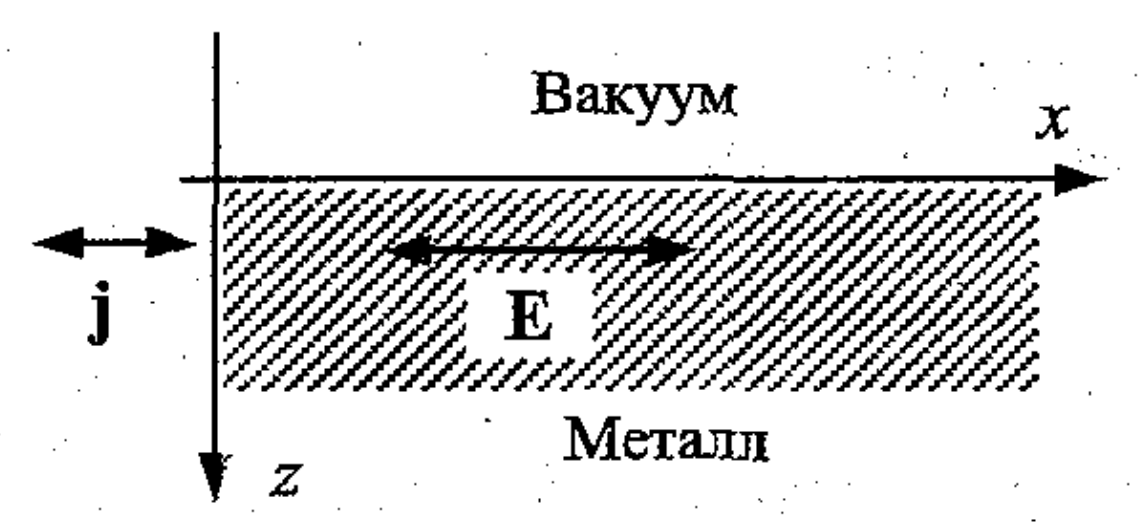
\includegraphics[width=0.4\textwidth]{../res/metal.png}
	\caption{}
	\label{fig:metal}
\end{wrapfigure}

Рассмотрим бесконечно большой, плоский проводник (рис. \ref{fig:metal}). Пусть вдоль границы проводника металл-вакуум течет переменный ток $J = J_0 cos \omega t$. Найдем объёмное распределение токов внутри проводника. В силу соображений симметрии и однородности проводника будем считать, что напряженность $E = E(z, t)$ и плотность тока $j = j(z, t)$ зависят только от расстояния до поверхности проводника $z$ и времени $t$.

Из уравнений Максвелла получим уравнение плоской электрической волны. Согласно закону Ома плотность тока $j$ связана с напряженностью электрического поля $E$ проводимостью $\sigma$ соотношением:
$$
\pmb{j} = \sigma \pmb {E}
$$
Далее будем предполагать, что характерная частота изменения поля достаточно мала, а проводимость металла велика, чтобы можно было пренебречь токами смещения по сравнению с токами проводимости. Также будем считать, что $\pmb{D} = \epsilon \epsilon_0 \pmb{E}$, $\pmb{B} = \mu \mu_0 \pmb{H}$ и в среде нет нескомпенсированных зарядов $\rho = 0$. Тогда уравнения Максвелла можно записать в виде:
\begin{equation*}
	\begin{split}
		\operatorname{rot} \pmb{E} &= -\mu \mu_0 \frac{\partial \pmb{H}}{\partial t} \\
		\operatorname{rot} \pmb{H} &= \pmb{j} = \sigma \pmb{E} \\
		\operatorname{div} \pmb{E} &= 0 \\
		\operatorname{div} \pmb{H} &= 0
	\end{split}
\end{equation*}
Применим операцию ротор к первому уравнению:
$$
\operatorname{rot} \operatorname{rot} \pmb{E} = - \mu \mu_0  \frac{\partial}{\partial t} \left( \sigma \pmb{E} \right)
$$
Из теории поля известно тождество:
$$
\operatorname{rot} \operatorname{rot} \pmb{E} = \operatorname{grad} \operatorname{div} \pmb{E} - \nabla^2 \pmb{E}
$$
Тогда получится уравнение плоской волны:
$$
\nabla^2 \pmb{E} = \mu \mu_0 \sigma \frac{\partial \pmb{E}}{\partial t}
$$
В одномерном случае $E = E(z, t)$ и волновое уравнение записывается в виде:
$$
\frac{\partial^2 E}{\partial z^2} = \mu \mu_0 \sigma \frac{\partial E}{\partial t}
$$
Для случая гармонических колебаний тока с частотой $\omega$, решения будем искать в виде:
$$
E(z, t) = E_0(z) \cdot e^{-i \omega t}
$$
Решением дифференциального уравнения будет
$$
E(z, t) = E_0(0) \exp{ \left( -\frac{z}{\Lambda} (1 - i) \right) }  \cdot \exp{ \left( -i \omega t \right) }
$$
Где введено обозначение $\Lambda = \sqrt{\frac{2}{\mu \mu_0 \sigma \omega}}$
Тогда распределение плотности тока внутри проводника будет равно
$$
j(z, t) = \sigma E(z, t) = j_0(0) \cdot \exp{ \left( -\frac{z}{\Lambda} \right)} \cdot \exp { \left( i \left(\frac{z}{ \Lambda} - \omega t \right) \right) }
$$
Проанализируем полученный результат. Ток в проводнике будет распределен по гармоническому закону с частотой $\omega$. На расстоянии $\Lambda$ от поверхности проводника амплитуда уменьшится в $e$ раз. То есть переменный ток $j$ и переменное электрическое поле $E$ проникают внутрь проводника на характерное расстояние $\Lambda$, называемое \textit{толщиной скин-слоя}. При увеличении частоты толщина скин-слоя уменьшается, поэтому высокочастотные токи будут распределены вдоль тонкого поверхностного слоя. В случае идеального проводника, когда $\lambda \rightarrow \infty$, $\Lambda \rightarrow 0$ токи тоже будут распределены по поверхности проводника.

\subsection*{Скин-эффект в полом цилиндре}

\begin{wrapfigure}{left}{0.32\textwidth}
	\vspace{-10pt}
	\centering
	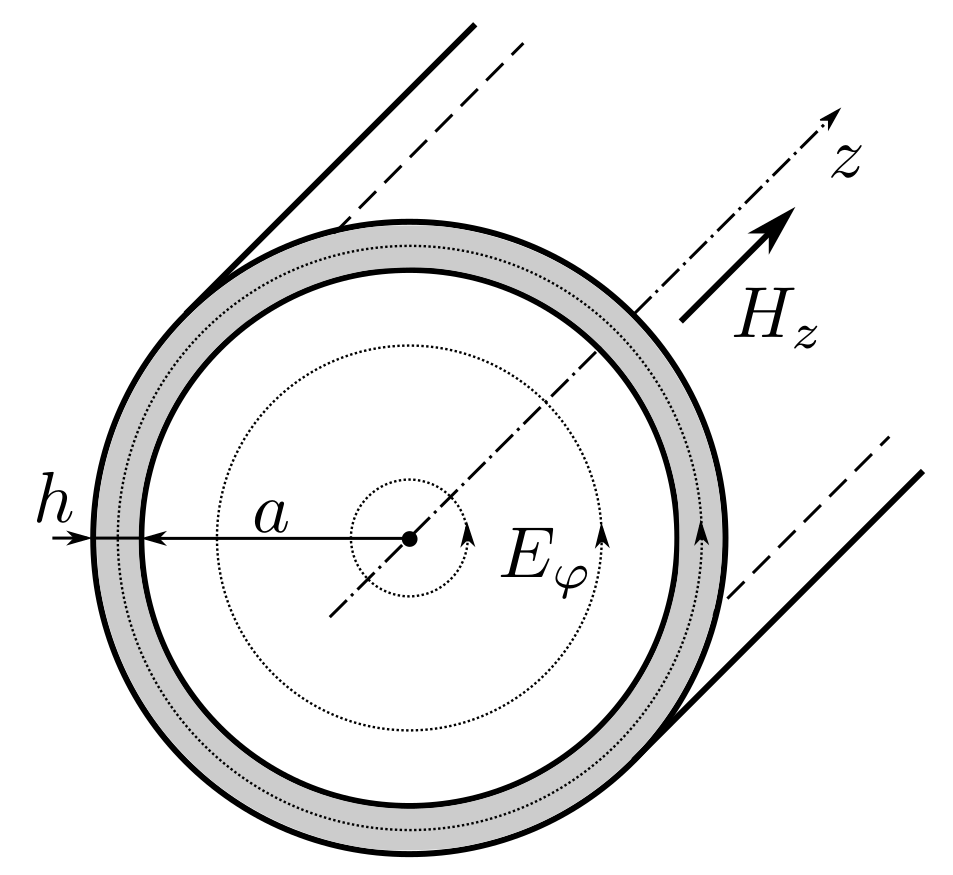
\includegraphics[width=0.3\textwidth]{../res/pipe.png}
	\caption{}
	\label{fig:pipe}
\end{wrapfigure}

В работе изучается скин-эффект в медном цилиндре, помещенном внутрь соленоида. Найти теоретическое распределение электромагнитного поля внутри такого цилиндра является сложной задачей, поэтому для упрощения вычислений и эксперимента используются следующие предположения. Цилиндр должен быть длинным, чтобы можно было пренебречь краевыми эффектами и считать электромагнитное поле зависящим только от расстояния до оси симметрии цилиндра. Так как измерить поле внутри твердого тела невозможно, то используется полый цилиндр. Измерив поле внутри цилиндра, можно вычислить поле на его границе. Чтобы можно было пренебречь кривизной стенок цилиндра и в малой области считать их плоскими, стенки цилиндра должны быть тонкими.

Магнитное поле внутри цилиндра направлено вдоль оси $z$, а вихревое электрическое поле всюду перпендикулярно радиусу. Пусть электромагнитное поле изменяется по гармоническому закону с частотой $\omega$:
\begin{equation*}
	\begin{split}
		H_z &= H(r) \cdot e^{i\omega t} \\
		E_{\phi} &= E(r) \cdot e^{i \omega t}
	\end{split}
\end{equation*}
На границе цилиндра касательные к поверхности компоненты как $\pmb{E}$, так и $\pmb{H}$ непрерывны. Так как внутри цилиндра ток отсутствует, то магнитное поле внутри цилиндра является однородным.
$$
H_z(r, t) = H_1 e^{i \omega t}
$$
По закону Фарадея найдем вихревое электрическое поле:
$$
E_{\phi} \cdot 2\pi r = - \pi r^2 \mu_0 \frac{d H_z}{dt} 
$$
$$
E(r) = -\frac{1}{2} \mu_0 r \cdot i\omega H_1
$$
На границе цилиндра $E_1 = -\frac{1}{2} i \omega a \mu_0 H_1$.

\begin{wrapfigure}{left}{0.32\textwidth}
	\vspace{-10pt}
	\centering
	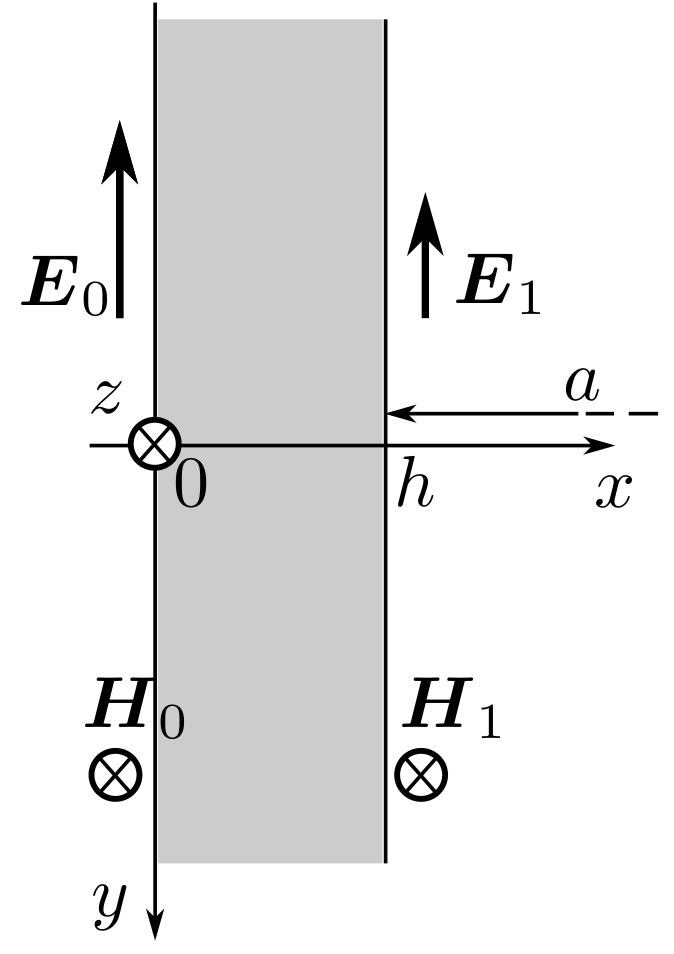
\includegraphics[width=0.3\textwidth]{../res/wall.png}
	\caption{Поле в стенке цилиндра}
	\label{fig:wall}
\end{wrapfigure}

Найдем распределение поля внутри стенки. Поле внутри стенки описывается уравнением скин-эффекта. 
$$
\frac{d^2 H}{dx^2} = i \omega \sigma \mu_0 H
$$
Зададим следующие граничные условия: 
\begin{equation*}
	\begin{split}
		H(0) &= H_0 \\
		H(h) &= H_1
	\end{split}
\end{equation*}
Решения будем искать в виде:
$$
H(x) = A e^{\alpha x} + B e^{-\alpha x}
$$
Решением дифференциального уравнения, удовлетворяющего данным начальным условиям будет
$$
H_1 = \frac{H_0}{\ch{ah} + \frac{1}{2} \alpha a \sh{\left( \alpha h \right)}}
$$
где $\alpha = \sqrt{i \omega \sigma \mu_0} = \frac{1 + i}{\Lambda}$.

Проанализируем предельные случаи.

\begin{figure}[H]
	\centering
	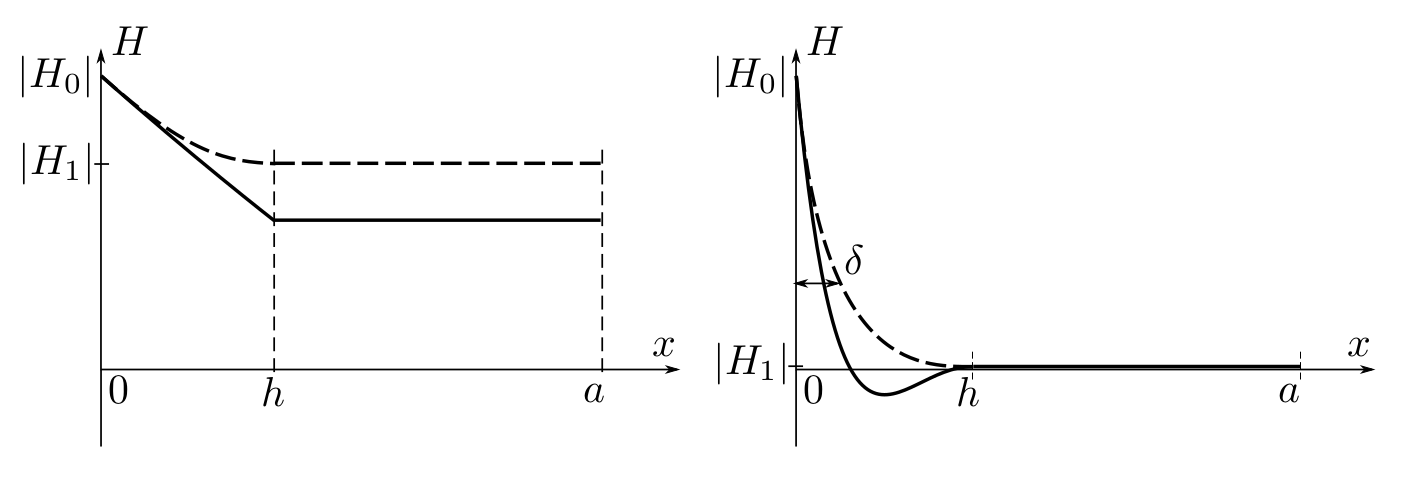
\includegraphics[width=0.7\textwidth]{../res/graphs.png}
	\caption{Распределение амплитуды колебаний магнитного поля изображено пунктиром, мгновенное значение в некоторый момент времени -- сплошной линией. Слева случай низких частот $\Lambda \gg h$, справа случай высоких частот $\Lambda \ll h$.}
	\label{fig:emi}
\end{figure}

\begin{enumerate}
	\item Случай низких частот $\Lambda \gg h$. Толщина скин-слоя превосходит толщину цилиндра, поэтому магнитное поле не полностью затухает внутри стенки цилиндра и имеет некую постоянную составляющую внутри полости. $\alpha h \ll 1$, $\ch{\alpha h} \approx 1$, $\sh{\alpha h} \approx \alpha h$.
	$$
	H_1 \approx \frac{H_0}{1 + i \frac{ah}{\Lambda^2}}
	$$
	Тогда отношение модулей амплитуд будет равно:
	$$
	\frac{|H_1|}{|H_0|} = \frac{1}{\sqrt{1 + \left( \frac{ah}{\Lambda} \right)^2}} = \frac{1}{\sqrt{1 + \frac{1}{4} \left( a h \sigma \mu_0 \omega \right)^2}}
	$$
	Колебания $H_1$ отстают по фазе от $H_0$ на угол $\varphi = \arctan \left( \frac{ah}{\Lambda} \right)^2 $.
	
	\item Случай высоких частот $\Lambda \ll h$. Толщина скин слоя меньше толщины стенки, поэтому внутри цилиндра магнитное поле будет равно 0. $\alpha h \gg 1$, $\sh{\alpha h} \approx \ch{\alpha h} \approx \frac{1}{2} e^{\alpha h}$.
	$$
	\frac{H_1}{H_0} = \frac{4}{\alpha a} e^{- \alpha h} = \frac{2\sqrt{2}\Lambda}{a} e^{-\frac{h}{\Lambda}} e^{-i \left( \frac{\pi}{4} + \frac{h}{\Lambda}\right)}
	$$
	Тогда отношение модулей амплитуд будет равно:
	$$
	\frac{|H_1|}{|H_0|} = \frac{2\sqrt{2}\Lambda}{a} e^{-\frac{h}{\Lambda}}
	$$
	Колебания $H_1$ отстают по фазе от $H_0$ на угол 
	\begin{equation}
		\varphi = \frac{\pi}{4} + \frac{h}{\Lambda}
		\label{formula:delta_phi}
	\end{equation}
\end{enumerate}

